\section{Overordnet Kravspecifikation}

\noindent
Systemet afspejler det system TV2 har lagt op til i projektcasen. Der er tale om et system, hvor alle kan se - og nogle kan redigere krediteringer for programmer. Systemet skal kunne tilgås via en dansk brugergrænseflade. Det skal indeholde forskellige brugerroller; systemadministrator, kanaladministrator, producer, royalty bruger og gæst.\\

\noindent
Systemadministratoren skal have rettigheder til at gøre alt. Dette gælder f.eks. at oprette krediteringer, kanaladministratorer og producerer. Kanaladministratoren skal kunne redigere, oprette og slette krediteringer for egen kanal. En producer skal kunne tilføje og redigere i krediteringerne for egne produktioner, og en gæst skal kunne se krediteringer for alle programmer. 
Det skal være muligt at kombinere personer som refererer til den samme person i den virkelige verden. Når to forskellige producere vil oprette en kreditering for et program, skal krediteringen være associeret med en person og vedkommendes rolle. Det betyder altså, at det skal være muligt at oprette personer der kan sammenflettes (f.eks. med UUID).\\

\noindent
TV2 har ikke lov til at lagre persondata, såsom et CPR-nummer eller et telefonnummer, så det skal være muligt at identificere personer i systemet og sikre at krediteringerne er korrekt forbundet til de rigtige personer.
Det skal være muligt at eksportere en specifik mængde data i forskellige formater såsom XML og CSV. Derudover skal databasen være søgbar, så det er nemt at finde personer, programmer og lignende. Det er vigtigt at systemet er nemt at bruge, så seerne nemt kan se krediteringerne for det program de lige har set.\\

\noindent
TV 2 kunne være interesseret i at integrere systemet med andre systemer (YouSee Tv, Boxer Play osv.), og det er derfor vigtigt at systemet er kompatibelt med krediteringer i andre systemer. Det kunne også være interessant at have muligheden for at få notifikationer når noget nyt sker i systemet. Samrådet for Ophavsret og Producentforeningen kunne også være interesseret i at modtage en form for meddelelse hver gang der er blevet tilføjet noget nyt til systemet, hvor de kan godkende krediteringerne og ud fra disse udbetale royalties. Derudover kunne det også være interessant at brugergrænsefladen kunne undestøtte flere sprog.\\

\noindent
For at beskytte dele af systemet (tilføjelse/redigering/sletning af data osv.), skal der indføres en form for adgangskontrol. Der skal være en offentligt tilgængelig del af systemet, hvor det er muligt at se krediteringerne for et et program uden at skulle logge ind.\\

\noindent
I tabel \ref{table:kravliste} ses kravene opsummeret i en tabel for bedre overblik.

\begin{longtable}[h]{ |p{1cm}|p{4cm}|p{11cm}| }

\hline
\textbf{ID} & \textbf{Navn} & \textbf{Beskrivelse} \\
\hline
K01 & Brugergrænseflade & Systemet skal tilgås via en dansk brugergrænseflade \\
\hline
K02 & Brugerroller & Systemet skal indeholde brugerroller \\
\hline
\label{K03}K03 & Tildel roller & Kanaladministrator skal kunne tildele producer- og kanaladministrator roller \\
\hline
K04 & Slet bruger & Systemadministratoren skal kunne slette brugere \\
\hline
K05 & Se krediteringer & Alle skal kunne se krediteringer \\
\hline
K06 & Søg efter krediteringer & Alle skal kunne søge efter og se krediteringer for alle programmer \\
\hline
K07 & Opret krediteringer & Specielle brugere, kanaladministratore og systemadmin skal kunne oprette
krediteringer for et givent program \\
\hline
K08 & Rediger krediteringer & Specielle brugere, kanaladmin og systemadmin skal kunne redigere krediteringer for egne programmer \\
\hline
K09 & Slet kreditering & Kanaladmin og systemadmin skal kunne oprette/redigere/slette krediteringer under egen kanal \\
\hline
K10 & Søg efter personer & Alle skal kunne søge efter personer \\
\hline
K11 & Knyt personer til krediteringer & Personer skal kunne knyttes til krediteringer så man kan se hvilke programmer en person har deltaget i Systemadmin, kanaladmin og producer skal kunne se persondata som email og tlf. nr. \\
\hline
K12 & Link personer i den virkelige verden & Det skal være muligt at linke personer i krediteringer til personer i den virkelige verden, så der krediteres korrekt \\
\hline
K13 & Eksporter data & Brugere skal kunne eksportere data til forskellige formater såsom XML og CSV \\
\hline
K14 & Importering af data & Systemet skal kunne importere EPG data via TVTid.dk \\
\hline
K15 & Integration & Systemet skal kunne integreres med andre systemer (Yoursee Play, Boxer Play, osv.) \\
\hline
K16 & Notifikationer & Systemet skal sende notifikationer til relevante brugere \\
\hline
K17 & Sprogvalg & Systemet skal kunne understøtte flere sprog \\
\hline
\caption{Liste af krav fra overordnet kravspecifikation} 
\label{table:kravliste}
\end{longtable} 

\subsection{Aktørliste}
Aktørlisten er sat op sådan, at overaktøren har samme rettigheder som underaktøren, samt ekstra rettigheder. F.eks. har systemadministratoren samme rettigheder som kanaladministratoren, plus rettigheder til at oprette kanaler, slette personer osv.\\


\begin{longtable}{|p{3.7cm}|p{6.15cm}|p{6.15cm}|}
\hline
\textbf{Aktør} & \textbf{Beskrivelse} & \textbf{Mål \& tjenester} \\
\hline
Systemadministrator (p) 
& Systemadministratoren har samme rettigheder som alle andre aktører. Denne aktør står primært for at slette personer, samt at oprette og slette kanaler. Til disse kanaler skal systemadministratoren tildele kanaladministratorroller.
& - Slette personer \newline - Oprette og slette kanaler \newline - Tildele og fjerne kanaladministratorroller\\

\hline
Kanaladministrator (p) 
& Kanaladministratoren skal godkende nyoprettede krediteringer, og har rettigheder til at slette krediteringer under egen kanal. Kanaladministratoren står får at tildele producer- og andre kanaladministratorroller for egen kanal.
& - Godkende nyoprettede krediteringer \newline - Slette krediteringer under egen kanal \newline - Tildele producer- og kanaladministratorroller for egen kanal\\

\hline
Royalty bruger (p) 
& Royalty bruger repræsenterer firmaer, som Registrering Danmark, der sørger for at betale royalties til medarbejdere på produktioner.
& - Kan eksportere data \\

\hline
Producer (p) 
& Produceren for et program står for at oprette nye krediteringer, samt rette krediteringer for egne produktioner.
& - Kan oprette krediteringer \newline - Kan redigere i eksisterende krediteringer for egne produktioner \newline - Kan logge ind og af \newline - Kan se personinformation \\

\hline
Gæst (p) 
& Gæsten repræsenterer offentligheden, som skal kunne søge efter informationer og krediteringer om forskellige programmer samt personer. Gæsten kan se alle produktioner en person har været med i. Gæsten kan også ændre sproget for brugergrænsefladen.
& - Kan søge efter og se krediteringer og personer for forskellige programmer \newline - Se alt hvad en person har været med i \newline - Ændre sproget\\

\hline
\caption{Aktørlisten}
\label{table:aktørlist}
\end{longtable}

\subsection{Overordnet Brugsmønstermodel}

\begin{figure}[H]
    \centering
    \captionsetup{justification=centering}
    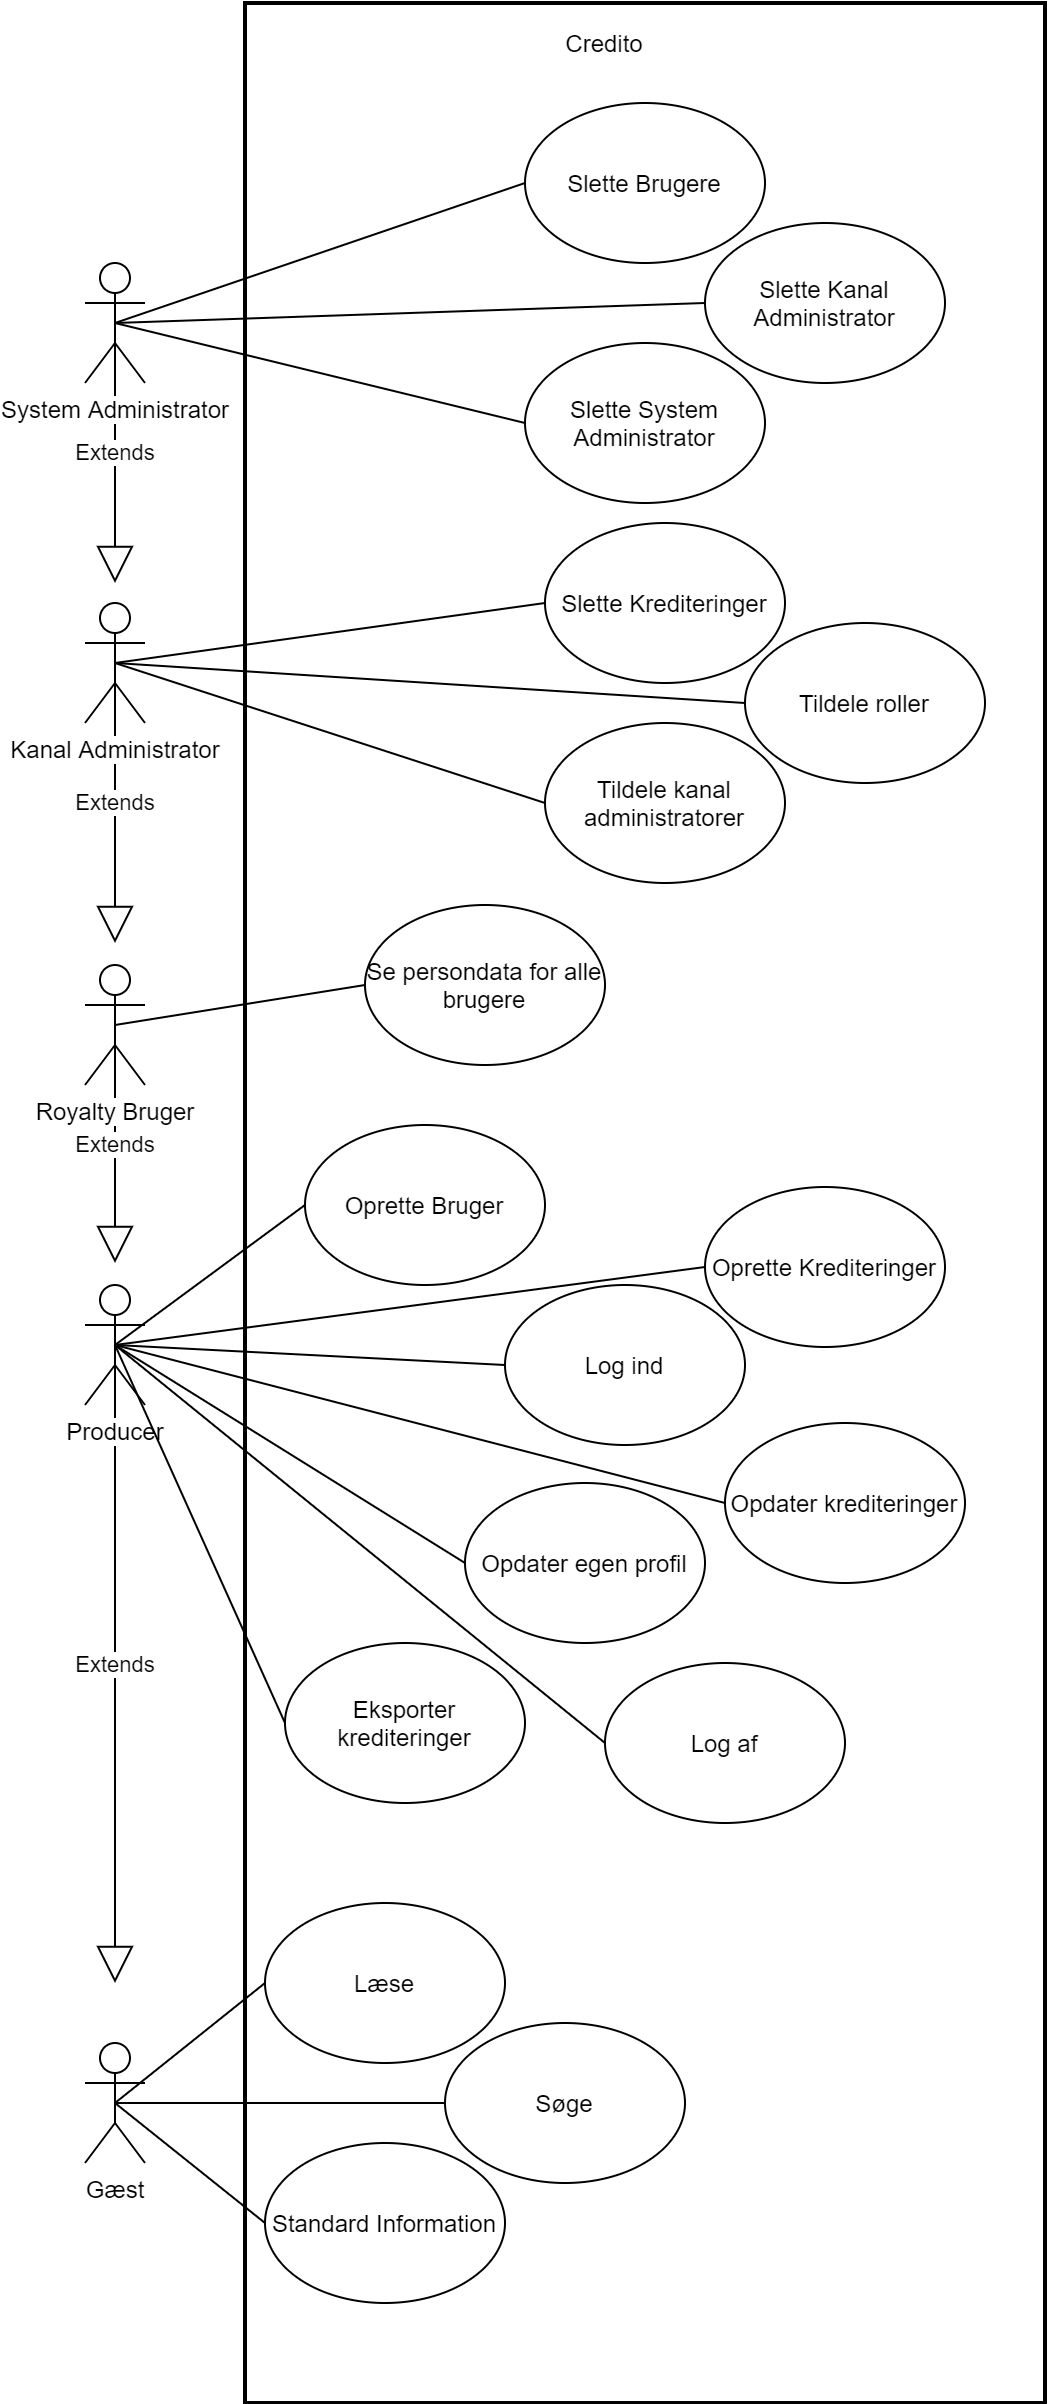
\includegraphics[scale=0.22]{figures/use-case.png}
    \caption[Overordnet brugsmønster over Creditoro systemet]%
    {Overordnet brugsmønster over Creditoro systemet 
    \par \small Menneskene er aktører. \\
    \small Cirklerne beskriver handlinger aktørne kan lave. \\
    \small Pilende betyder Extends, hvilket vil sige aktørerne arver funktionalitet}
    \label{fig:usecasemodel}
\end{figure}

\newpage
\subsection{Liste over Brugsmønstre}

\begin{longtable}[h]{|p{0.6cm}|p{6.4cm}|p{9cm}| }
\hline
\textbf{ID} & \textbf{Navn} & \textbf{Aktør} \\
\hline
B01 & Opdater egen royalty bruger & Systemadministrator (p), Royalty Bruger (p) \\
\hline
B02 & Opdater person & Systemadministrator (p), kanaladministrator (p), producer (p) \\
\hline
B03 & Opret Producer & Systemadministrator (p), kanaladministrator (p) \\
\hline
B04 & Opret person & Systemadministrator (p), kanaladministrator (p), Producer (p) \\
\hline
B05 & Fjern producer & Systemadministrator (p) \\
\hline
B06 & Fjern person & Systemadministrator (p) \\
\hline
B07 & Opret kreditering & Systemadministrator (p), Kanaladministrator (p), producer (p) \\
\hline
B08 & Fjern kreditering til program & Systemadministrator (p), kanaladministrator (p) \\
\hline
B09 & Opdater egne kreditering & Systemadministrator (p), kanaladministrator (p), Producer (p) \\
\hline
B10 & Læse krediteringer & Systemadministrator (p), kanaladministrator (p), Royalty Bruger (p), Producer (p), Gæst (p) \\
\hline
B11 & Se person profil & Systemadministrator (p), kanaladministrator (p), Royalty bruger (p), Producer (p), Gæst (p) \\
\hline
B12 & Søge efter personer og programmer & Systemadministrator (p), kanaladministrator (p), Royalty Bruger (p), Producer (p), Gæst (p) \\
\hline
B13 & Log ind & Systemadministrator (p), kanaladministrator (p), Royalty Bruger (p), Producer (p) \\
\hline
B14 & Log af & Systemadministrator (p), kanaladministrator (p), Royalty Bruger(p), Producer (p) \\
\hline
B15 & Kan se personinformation & Systemadministrator (p), kanaladministrator (p), Royalty Bruger (p), Producer (p) \\
\hline
B16 & Godkende nye krediteringer & Systemadministrator (p), Kanaladministrator (p) \\
\hline
B17 & Afvise nye krediteringer & Systemadministrator (p), Kanaladministrator (p) \\
\hline
B18 & Opret kanaladministrator & Systemadministrator (p), kanaladministrator (p) \\
\hline
B19 & Opret systemadministrator & Systemadministrator (p) \\
\hline
B20 & Ændre sprog & Systemadministrator (p), kanaladministrator (p), Royalty Bruger (p), Producer (p), Gæst (p) \\
\hline
\caption{Brugsmønstre}
\label{tab:brugsmønstre}
\end{longtable}

\newpage
\subsection{Overordnet Supplerende Krav}

Her bruges FURPS for supplerende krav.
\begin{table}[H]
    \centering
    \begin{tabular}{|p{3cm}|p{13cm}|}
    \hline
    \textbf{FURPS}           &    \textbf{Krav} \\
    \hline
    %What the customer wants! Note that this includes security-related needs.
    Functionality           & Skal kunne kreditere produktionsroller som er angivet af DRs Krediteringsregler \\
                            & Skal overholde GDPR \\
    \hline
    % How effective is the product from the standpoint of the person who must use it? Is it aesthetically acceptable? Is the documentation accurate and complete?
    Usability       & Systemet skal kunne understøtte flere sprog \\
    \hline
    % What is the maximum acceptable system downtime? Are failures predictable? Can we demonstrate the accuracy of results? How is the system recovered?
    Reliability     &  Hvis serveren til systemet genstarter, startes del-systemerne igen automatisk. Der vil ikke være behov for at ligge systemet ned regelmæssigt for at kunne foretage backup. \\
    \hline
    % How fast must it be? What's the maximum response time? What's the throughput? What's the memory consumption?
    Performance     &  Databasen skal kunne håndtere 10000 nye brugere - samt 15000 krediteringerer årligt i 25 år, uden at ofte brugte kald til REST Api'et bliver sløvt (reponsetid på mere end 300 ms) \\
    \hline
    % Is it testable, extensible, serviceable, installable, and configurable? Can it be monitored?
    Supportability  &  Systemet vil indeholde unit tests, og komme med en rapport over hvor stor en procendel der er dækket af dette. % Hvis der er mere tid kan vi indrage integrations tests?
    %Centraliseret logning (Elastic search, eller blot centraliseret system log?)
    Systemet vil blive forbundet til det centraliserede fejllognings system \texttt{Sentry}.
    Systemet er installerbart vha. Docker via Docker-compose. % (så vi blot kan sige docker-compose up -d for at få systemet op).
    Det vil være muligt at konfigurere system indstillinger via en \texttt{.env} (miljø) fil.
    En opsætningsguide vil være at finde sammen med kildekoden. 
    \\ \hline
    % The + reminds us of a few additional needs that a customer could have:
    % fx. Design constraints, Implementation requirements, interface requirements or physical requirements.
    \end{tabular}
    \caption{FURPS}
    \label{tab:furps}
\end{table} 


\subsection{Detaljerede Beskrivelse af Udvalgte Essentielle Brugsmønstre}
Ud fra MoSCoW har vi valgt 2 brugsmønstre vi mener er essentielle for systemet. De to brugsmønstre er 'Læs kreditering' og 'Opret kreditering'. Til disse to brugsmønstre har vi lavet detaljerede brugsmønstre som kan ses i tabel \ref{table:read_credits} og tabel \ref{tab:create_credits}.

\begin{longtable}[h]{|p{16cm}|}
    \hline
    \textbf{Brugsmønster:}  Læs kreditering \\ 
    \hline
	\textbf{ID:} UC10 \\ 
	\hline
	\textbf{Primære aktører:} Systemadministrator, kanaladministrator, producer, royalty bruger, gæst \\ \hline
	\textbf{Sekundære aktører:} \\ \hline
	\textbf{Kort beskrivelse:} Alle skal kunne se krediteringen for programmerne. \\ \hline
	\textbf{Prækonditioner (Pre conditions):} \\ \hline
\textbf{Hovedhændelsesforløb (main flow):} \\
1. Brugsmønstret starter når en aktør vil se kredit for et program \\
2. Aktøren søger efter programmet \\
3. Aktøren trykker på det ønskede program \\
4. Systemet checker hvilken rolle aktøren har \\
5. Aktøren bliver omdirigeret til den passende visning af krediteringen \\ \hline
    \textbf{	Postkonditioner (post conditions):} \\
    En kreditering bliver vist \\ \hline

	\textbf{Alternative hændelsesforløb (alternative flow):} \\
Step 2: Hvis programmet ikke findes, får vedkommende besked om at programmet ikke findes \\ 
\hline
\caption{Brugsmønster: Læs kreditering}
\label{table:read_credits}
\end{longtable}

% Kevin something fishy here
% Skal det ikke være tabular?
\begin{longtable}[h] {|p{16cm}|}
\hline
    \textbf{Brugsmønster:} Opret kreditering \\
    \hline
	\textbf{ID:} UC07 \\ \hline
	\textbf{Primære aktører:} Systemadministrator, kanaladministrator, Producer \\ \hline
	\textbf{Sekundære aktører:} \\ \hline
	\textbf{Kort beskrivelse:} Produceren opretter en kreditering. Heri angives alle der har bidraget til produceringen af TV-programmet, filmen el. lign. \\ \hline
	\textbf{Prækonditioner (Pre conditions):} \\
Aktøren skal være logget på systemet \\ \hline
\textbf{Hovedhændelsesforløb (main flow):} \\
	1. Brugsmønstret starter når en administrator eller producer vil oprette en kreditering \\
	2. Aktøren trykker på knappen ‘Opret Kreditering’ \\
	3. Systemet checker aktørens rolle \\
	4. Aktøren er forbundet til en kanal, og angiver programmets titel \\
	5. Systemet checker om der allerede findes et program med den angivne \\ titel
	6. Aktøren krediterer alle der har medvirket i produktionen af \\ programmet
	7. Aktøren sender den færdige kreditering videre til godkendelse \\
	8. Postkonditioner (post conditions): \\
	9. En kreditering er blevet oprettet \\ \hline
	\textbf{Alternative hændelsesforløb (alternative flow):} \\
Step *: Aktøren kan til enhver tid afbryde oprettelsen af krediteringen \\
Step 4: Hvis aktøren er systemadministrator, er vedkommende ikke forbundet til en kanal, og kan skifte hvilken kanal krediteringen skal oprettes ved. \\

Step 5: Hvis programmets titel allerede eksistere, gøres aktøren opmærksom på dette. \\

Step 8: Hvis krediteringen afvises, laves de fornødne ændringer, og den nye kreditering sendes videre til godkendelse. \\
\hline
\caption{Brugsmønster: Opret kreditering}
\label{tab:create_credits}
\end{longtable}